\documentclass{beamer}
\usepackage[utf8]{inputenc}

\usetheme{Madrid}
\usecolortheme{default}
\usepackage{amsmath,amssymb,amsfonts,amsthm}
\usepackage{txfonts}
\usepackage{tkz-euclide}
\usepackage{listings}
\usepackage{adjustbox}
\usepackage{array}
\usepackage{tabularx}
\usepackage{gvv}
\usepackage{lmodern}
\usepackage{circuitikz}
\usepackage{tikz}
\usepackage{graphicx}
 \graphicspath{{figs/}}
\setbeamertemplate{page number in head/foot}[totalframenumber]
\usepackage[T1]{fontenc}
\usepackage{lmodern}

\usepackage{tcolorbox}
\tcbuselibrary{minted,breakable,xparse,skins}



\definecolor{bg}{gray}{0.95}
\DeclareTCBListing{mintedbox}{O{}m!O{}}{%
  breakable=true,
  listing engine=minted,
  listing only,
  minted language=#2,
  minted style=default,
  minted options={%
    linenos,
    gobble=0,
    breaklines=true,
    breakafter=,,
    fontsize=\small,
    numbersep=8pt,
    #1},
  boxsep=0pt,
  left skip=0pt,
  right skip=0pt,
  left=25pt,
  right=0pt,
  top=3pt,
  bottom=3pt,
  arc=5pt,
  leftrule=0pt,
  rightrule=0pt,
  bottomrule=2pt,
  toprule=2pt,
  colback=bg,
  colframe=orange!70,
  enhanced,
  overlay={%
    \begin{tcbclipinterior}
    \fill[orange!20!white] (frame.south west) rectangle ([xshift=20pt]frame.north west);
    \end{tcbclipinterior}},
  #3,
}
\lstset{
    language=C,
    basicstyle=\ttfamily\small,
    keywordstyle=\color{blue},
    stringstyle=\color{orange},
    commentstyle=\color{green!60!black},
    numbers=left,
    numberstyle=\tiny\color{gray},
    breaklines=true,
    showstringspaces=false,
}
%------------------------------------------------------------
%This block of code defines the information to appear in the
%Title page
\title %optional
{1.8.24}
%\subtitle{A short story}

\author % (optional)
{Aniket-EE25BTECH11007}

\begin{document}
\frame{\titlepage}

\begin{frame}{Question}
If $(a,b)$ is the mid-point of the line segment joining the point 
$\vec{A}$ $(10,-6)$ and $\vec{B}$ $(k,4)$ and $a-2b=18$, find the value of $a,b$ and the distance $\vec{AB}$.\\
\end{frame}
\begin{frame}{Theoretical Solution}
Let
\(\vec{A}=\myvec{x_1\\ y_1}\) and \(\vec{B}=\myvec{x_2\\ y_2}\).
By the (matrix) section formula, the point dividing \(\vec{A}\vec{B}\) in the ratio \(k:1\) is
\begin{equation}
R_{\text{int}}=\frac{1}{k+1}[\,\vec{A}\;\vec{B}\,]\myvec{1\\ k}.
\end{equation}

\medskip

With \(\vec{A}=\myvec{10\\-6}\) and \(\vec{B}=\myvec{k\\4}\) and \(\vec{O}=\myvec{a\\b}\) the midpoint (\(k=1\)) is
\begin{equation}
\vec{O}=\frac12[\,\vec{A}\;\vec{B}\,]\myvec{1\\1}
=\frac12\myvec{10 & k\\[2pt] -6 & 4}\myvec{1\\1}
=\myvec{\dfrac{10+k}{2}\\[6pt]-1}.
\end{equation}

\end{frame}
\begin{frame}{Theoretical Solution}
Thus,
\begin{align}
a &= \frac{10+k}{2}, \quad b = -1 \tag{3}
\end{align}

Using the given condition $a - 2b = 18$:
\begin{align}
\frac{10+k}{2} - 2(-1) &= 18 \tag{4}\\
k &= 22 \tag{5}
\end{align}

So,
\begin{align}
a = \boxed{16}, \quad b = \boxed{-1} \tag{6}
\end{align}
\end{frame}
\begin{frame}{Theoretical Solution}
\textbf{Distance Between \(\vec{A}\vec{B}\):}

\[
\|\vec{A}-\vec{B}\|=\sqrt{(\vec{A}-\vec{B})^{\top}(\vec{A}-\vec{B})}. \tag{7}
\]

Given,
\[
\vec{A}=\myvec{10\\-6},\qquad \vec{B}=\myvec{22\\4}. \tag{8}
\]



\begin{align}
\|\vec{A}-\vec{B}\| &= \sqrt{(-12)^2+(-10)^2} \tag{9} \\
                    &= \boxed{2\sqrt{61}} \tag{10}
\end{align}


\end{frame}


\begin{frame}[fragile]
    \frametitle{C Code - Finding Midpoint and Distance between 2 points}

    \begin{lstlisting}
#include <stdio.h>
#include <math.h>

// Solve the midpoint + constraint problem
// A = (Ax, Ay)
// B = (k, By)   (Bx is unknown, denoted k)
// Constraint:   p*a + q*b = r,  where (a,b) is midpoint
//
// Outputs:
//   *a, *b  → midpoint coordinates
//   *k      → solved x-coordinate of B
//   *ABx,*ABy → vector A-B
//   *norm2  → squared distance (A-B).(A-B)
void solve_problem(double Ax, double Ay, double By,
                   double p, double q, double r,
                   double *a, double *b, double *k,
                   double *ABx, double *ABy, double *norm2)
\end{lstlisting}
\end{frame}

                   \begin{frame}[fragile]
    \frametitle{C Code - Finding Midpoint and Distance between 2 points}

    \begin{lstlisting}
{
    // Midpoint coordinates
    *b = (Ay + By) / 2.0;
    *k = (2.0 * r - p * Ax - 2.0 * q * (*b)) / p;
    *a = (Ax + *k) / 2.0;

    // Vector A - B
    *ABx = Ax - *k;
    *ABy = Ay - By;

    // Squared distance
    *norm2 = (*ABx) * (*ABx) + (*ABy) * (*ABy);
}
\end{lstlisting}
\end{frame}

\begin{frame}[fragile]
    \frametitle{Python+C Code}
    \begin{lstlisting}

    import ctypes
import numpy as np
import matplotlib.pyplot as plt

# Load shared object
lib = ctypes.CDLL("./mg2.so")

# Define argument and return types
lib.solve_problem.argtypes = [
    ctypes.c_double, ctypes.c_double, ctypes.c_double,  # Ax, Ay, By
    ctypes.c_double, ctypes.c_double, ctypes.c_double,  # p, q, r
    ctypes.POINTER(ctypes.c_double), ctypes.POINTER(ctypes.c_double), ctypes.POINTER(ctypes.c_double),
    ctypes.POINTER(ctypes.c_double), ctypes.POINTER(ctypes.c_double), ctypes.POINTER(ctypes.c_double)
]
\end{lstlisting}
\end{frame}

\begin{frame}[fragile]
    \frametitle{Python+C Code}
    \begin{lstlisting}

lib.solve_problem.restype = None

# Inputs
Ax, Ay = 10.0, -6.0
By = 4.0
p, q, r = 1.0, -2.0, 18.0   # constraint: a - 2b = 18

# Outputs (ctypes)
a = ctypes.c_double()
b = ctypes.c_double()
k = ctypes.c_double()
ABx = ctypes.c_double()
ABy = ctypes.c_double()
norm2 = ctypes.c_double()

\end{lstlisting}
\end{frame}
\begin{frame}[fragile]
    \frametitle{Python+C Code}
    \begin{lstlisting}
# Call C function
lib.solve_problem(
    Ax, Ay, By, p, q, r,
    ctypes.byref(a), ctypes.byref(b), ctypes.byref(k),
    ctypes.byref(ABx), ctypes.byref(ABy), ctypes.byref(norm2)
)

# Convert results into NumPy arrays
A = np.array([Ax, Ay])
B = np.array([k.value, By])
O = np.array([a.value, b.value])

print("A =", A)
print("B =", B)
print("O (midpoint) =", O)
print("Vector A-B =", A - B)
print("Squared distance =", norm2.value)
\end{lstlisting}
\end{frame}
\begin{frame}[fragile]
    \frametitle{Python+C Code}
    \begin{lstlisting}

# Plotting
plt.figure()
plt.plot([A[0], B[0]], [A[1], B[1]], 'k-')  # segment AB
plt.scatter(*A, color='red', label='A')
plt.scatter(*B, color='blue', label='B')
plt.scatter(*O, color='green', label='Midpoint O')

plt.text(A[0]+0.5, A[1], f"A{tuple(A.astype(int))}")
plt.text(B[0]+0.5, B[1], f"B{tuple(B.astype(int))}")
plt.text(O[0]+0.5, O[1], f"O{tuple(O.astype(int))}")

plt.gca().set_aspect('equal', adjustable='box')
plt.legend()
plt.title("Segment AB and Midpoint O")
plt.show()

\end{lstlisting}
\end{frame}

\begin{frame}[fragile]
    \frametitle{Python Code}
    \begin{lstlisting}

    import numpy as np
import matplotlib.pyplot as plt

# Given data
A = np.array([10, -6])
B = np.array([22, 4])
O = (A + B) // 2   # midpoint (integer division gives exact midpoint here)

# Convert to Python tuples for clean display
A_t = tuple(A.tolist())
B_t = tuple(B.tolist())
O_t = tuple(O.tolist())
\end{lstlisting}
\end{frame}
\begin{frame}[fragile]
    \frametitle{Python Code}
    \begin{lstlisting}

# Print results
print("A =", A_t)
print("B =", B_t)
print("O =", O_t)

# Plotting
plt.figure()
plt.plot([A[0], B[0]], [A[1], B[1]], 'k-', label="Segment AB")  # line AB
plt.scatter(*A, color='red', label=f"A{A_t}")
plt.scatter(*B, color='blue', label=f"B{B_t}")
plt.scatter(*O, color='green', label=f"O{O_t}")
\end{lstlisting}
\end{frame}
\begin{frame}[fragile]
    \frametitle{Python Code}
    \begin{lstlisting}

# Annotate points with clean integer tuples
plt.text(A[0]+0.5, A[1], f"A{A_t}")
plt.text(B[0]+0.5, B[1], f"B{B_t}")
plt.text(O[0]+0.5, O[1], f"O{O_t}")

plt.gca().set_aspect('equal', adjustable='box')
plt.legend()
plt.title("Segment AB and Midpoint O")
plt.xlabel("x-axis")
plt.ylabel("y-axis")
plt.grid(True)
plt.show()

\end{lstlisting}
\end{frame}

\begin{frame}{Plot}
    \centering
    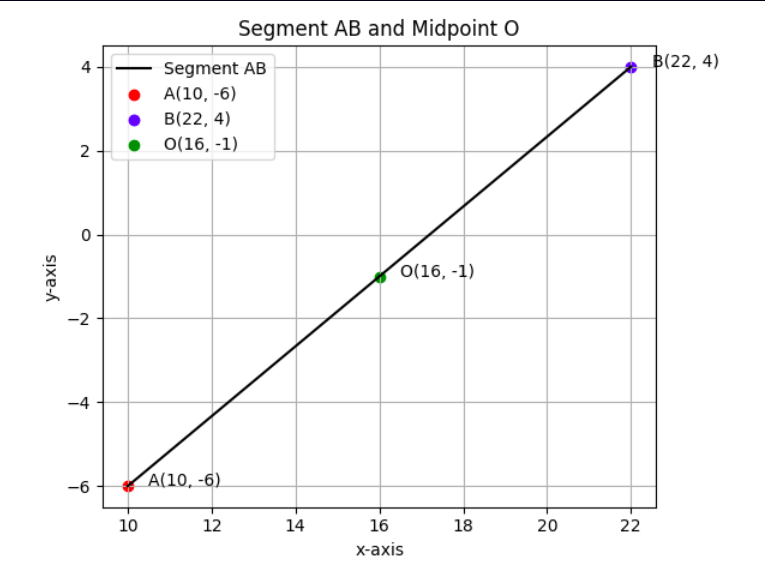
\includegraphics[width=\columnwidth, height=0.8\textheight, keepaspectratio]{figs/mg2.png}     
\end{frame}



\end{document}